\chapter{Desenvolvimento do modelo OLAP}
%-------------------------------------------------------
% descrever como foi feito o levantamento dos residuos mais interesantes. 
%  Explicar que a lista dos mais presentes foi comparada com uma lista originalmente desenvolvida por um especialista de dominio. 
%  Encontrou se casos que estavam e nao estavam na lista, os que nao apareciam na lista constituem de residuos que se ficam ˜proximos”ao sitio de ligação, mas que na realidade estão fora do sítio.
% descrever como  adicionar novas dimensoes baseadas em novos residuos
%-------------------------------------------------------

Para possibilitar a construção do modelo OLAP, primeiramente foi necessário identificar e definir as questões de negócio que seriam relevantes sob o ponto de vista do especialista de domínio. Em virtude disso, o levantamento destes dados foi feito por meio de entrevistas com os especialistas do LABIO.

A Tabela \ref{tab:questaoNegocio} descreve as questões de negócio que foram identificadas como sendo mais relevantes para execução de análise de experimentos de docagem realizados no LABIO. 

\begin{table}[h]
\caption{Questões de negócio identificadas pelos especialistas com maior relevância para análise de experimentos de docagem}
\label{tab:questaoNegocio}
\centering
\begin{tabular}{@{}ll@{}}
\toprule
\textbf{ } & \multicolumn{1}{c}{\textbf{Questões de maior relevância para a análise de docagem}}		\\ \midrule
\textbf{1.} & Associar um grupo para cada conformação;													\\
\textbf{2.} & Identificar o comportamento das conformações baseado nas métricas de FEB e RMSD;			\\
\textbf{3.} & Identificar conformações/grupos que possuem o maior número de contatos com os ligantes;	\\
\textbf{4.} & Com base no item 3, identificar quais são os resíduos mais importantes;					\\
\textbf{5.} & Com base no item 3, identificar quais grupos possuem melhores valores de FEB e RMSD.		\\ \bottomrule
\end{tabular}
\end{table}

\section{Identificação de métricas}

Durante as entrevistas realizadas, pode-se perceber que informações baseadas nas métricas de FEB e RMSD possuíam grande relevância para responder as questões de negócio. Entretanto foi necessário definir certas propriedades e limitações de valores para adequar os cálculos às necessidades do negócio. Dessa maneira, todas as definições citadas nesta seção foram estabelecidas em conjunto com os especialistas de domínio do LABIO, para que os resultados apresentados pudessem representar a realidade.

O cálculo da FEB é um dos métodos utilizados pelos softwares de docagem que permite avaliar a interação receptor-ligante. Quanto menor for o resultado deste cálculo, mais favorável é a ligação estabelecida. Portanto, o valor estimado da FEB é utilizado como uma das métricas do modelo.

Na maioria dos experimentos, os melhores resultados de FEB são valores negativos. Portanto, qualquer conformação que apresente valores de FEB positivos não foram levados em consideração. Dessa maneira evita-se que os resultados positivos venham a interferir em uma análise futura dos valores agregados de um experimento. 

O cálculo do RMSD é utilizado para obter a distância média entre os átomos. Nos experimentos de docagem, este cálculo é feito para comparar o posicionamento inicial do ligante, geralmente estipulada pelo especialista de domínio, com o posicionamento final após a execução da docagem. Neste caso, o RMSD é considerado como uma métrica para a modelagem.

Tanto a FEB quando o RMSD dão uma visão para o especialista de quão satisfatório foi o processo de docagem para uma determinada iteração. Enquanto a FEB mede a qualidade da docagem no aspecto termodinâmico da questão, o RMSD tem como natureza avaliar geometricamente como estão dispostas as moléculas do resíduo e do ligante.

Além disso, para ser possível responder ao item 3 da Tabela \ref{tab:questaoNegocio}, foi necessário incluir uma métrica para contabilizar o número de contatos entre o ligante e um resíduo da molécula receptora. 

Um contato pode ser identificado pelo cálculo da medida em {\AA}ngstr\"om entre os átomos do resíduo do receptor e do ligante. Ou seja, para cada resíduo do receptor \emph{R} é calculada a distância Euclidiana entre todos seus átomos e os átomos de um ligante \emph{L}. Sendo $R=(r_{x},r_{y},r_{z})$ representando as coordenadas dos átomos dos resíduos do receptor, e $L=(l_{x},l_{y},l_{z})$ representando as coordenadas dos átomos do ligante, o cálculo da distância se dá pela equação \ref{eqt:distEuclid}.

\begin{equation}
\label{eqt:distEuclid}
	d(R,L)=\sqrt{(r_{x}-l_{x})^{2}+(r_{y}-l_{y})^{2}+(r_{z}-l_{z})^{2}}
\end{equation}

Em suma, para cada snapshot devem ser calculadas todas as coodernadas do receptor com todas as coordenadas de cada ligante, neste caso para o TCL e para o ETH. Entretanto, de todas as distâncias calculadas para um resíduo, apenas a menor delas deve ser considerada. 

A Figura \ref{fig:PIFvsGLY} ilustra este conceito, apresentando como exemplo as distâncias entre os átomos do ligante PIF (cor preto) e do resíduo GLY95 (cor cinza) do receptor InhA. Para todas as distâncias calculadas, a menor delas é de 2.72 {\AA} \cite{MAC10}.

\begin{figure}[h]
	\center
	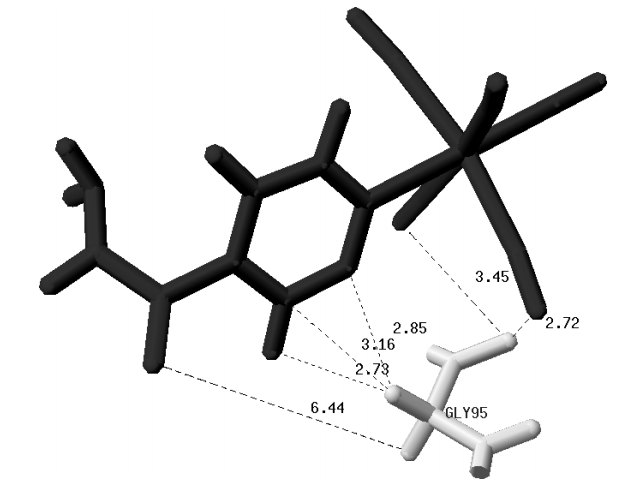
\includegraphics[scale=0.5]{images/distEucli.png}
	\caption{Cálculo das distâncias atômicas entre o ligante PIF (cor preta) e o resíduo GLY95 (cor cinza) do receptor InhA \cite{MAC10}.}
	\label{fig:PIFvsGLY}
\end{figure} 

\section{Identificação dos resíduos relevantes}
%-------------------
% TO DO: explicar como foi feito o cálculo para obter o número de contatos
%        descrever limitação de 2 e 4 angstrons.
%-------------------

Um dos pontos mais importantes para responder aos questionamentos dos especialistas de domínio e fundamental para composição das dimensões, era saber quais eram os resíduos mais relevantes. A enzima InhA possui 268 resíduos \cite{KARANADUNOSM09} e o processo de identificação dos mais importantes leva em consideração o número de contatos do resíduo com o ligante. Na base de informações que foi resultado do processo de simulação de docagem, cada resíduo é representado por uma tripla contendo a sua localização espacial nos eixos x, y e z.

De acordo com o especialista de domínio, para ser considerado contato do resíduo com o ligante é preciso estar em uma distância entre 2 e 4 angstrom. Valores inferiores a 2 angstrom são descartados por serem considerados uma sobreposição. Desta forma é utilizado o cálculo da distância euclidiana entre os átomos do resíduo e do ligante \cite{KARANADUNOSM09} para encontrar estes valores, desprezando os átomos de hidrogênio conforme determinação dos especialistas de domínio. Quanto maior o número de contatos do resíduo com o ligante, mais relevante para o especialista é o resíduo. As regras para elencar os resíduos mais relevantes podem ser sumarizadas da seguinte forma:

\begin{enumerate}
    \item Distância de 2 a 4 angstrom são considerados contatos.
    \item Distância inferior a 2 angstrom são desconsideradas. 
    \item Descarte do cálculo para os átomos de hidrogênio.
    \item Quanto mais contatos, mais relevante.
\end{enumerate}

Após execução dos algoritmos elaborados dentro do trabalho para coletar estas informações, foram identificados 15 resíduos mais relevantes que posteriormente foram avaliados pelos especialistas e reduzidos a uma lista de 10 resíduos. Com base em uma lista anteriormente elaborada por um especialista de domínio, conforme mostrado na Figura \ref{fig:ListaOsmar}, os 5 resíduos que sobraram dos 15 iniciais foram identificados como casos onde a proteína, devido a flexibilidade, abriu uma cavidade acima da cavidade do substrato, permitindo ligações do ligante fora da cavidade do substrato.

\begin{figure}[h]
        \center
        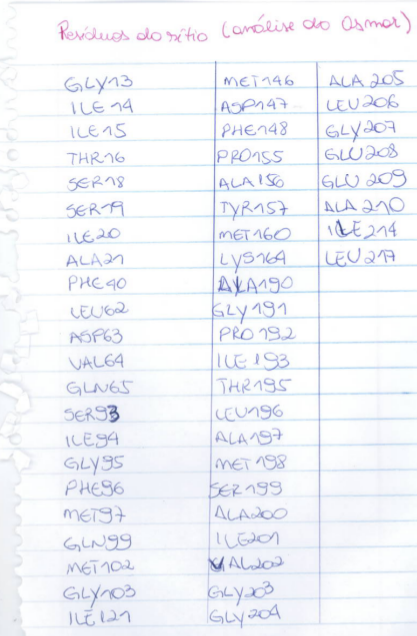
\includegraphics[width=12cm]{images/ListaProfOsmar.png}
        \label{fig:ListaOsmar}
        \caption{Lista dos principais resíduos do Professor Osmar}
\end{figure}

A Figura \ref{fig:PlotResiduos} mostra os 15 resíduos que foram identificados inicialmente. Aqueles indicados em vermelho são os considerados importantes e os indicados em branco foram descartados porque ficaram fora do sítio de ligação.

\begin{figure}[h]
        \center
        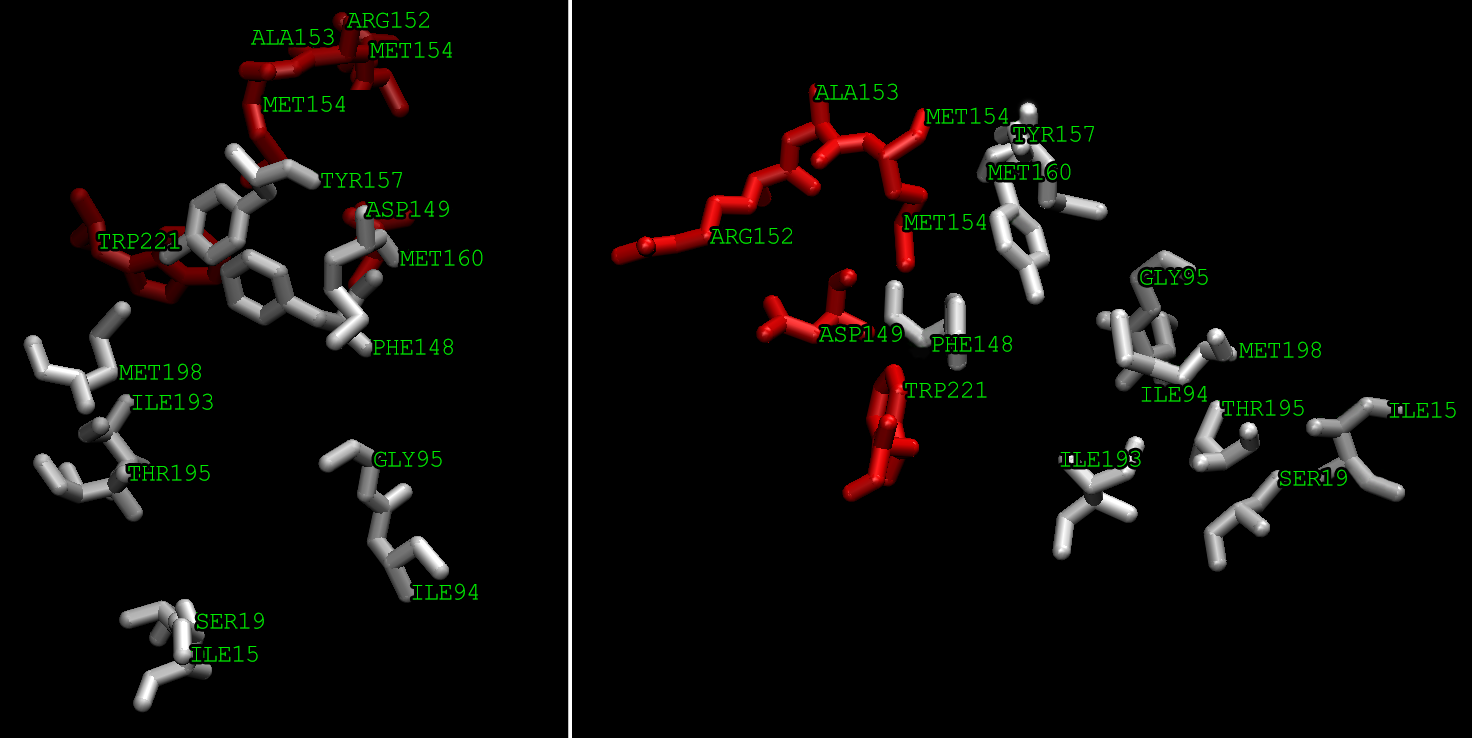
\includegraphics[width=10cm]{images/avaliacao_Residuos_nomes.png}
        \label{fig:PlotResiduos}
        \caption{Lista inicial dos 15 resíduos mais relevantes}
\end{figure}

Com base nestas prerrogativas foram selecionados os 10 principais resíduos mais relevantes para responder às questões dos especialistas conforme mostrado.

\begin{itemize}
	\item PHE\_148 (Phenylalanine)
	\item ILE\_193 (Isoleucine)
	\item GLY\_95 (Glycine)
	\item THR\_195 (Threonine)
	\item ILE\_94 (Isoleucine)
	\item MET\_198 (Methionine)
	\item MET\_160 (Methionine)
	\item SER\_19 (Serine)
	\item ILE\_15 (Isoleucine)
	\item TYR\_157 (Tyrosine)
\end{itemize}

\section{Scripts para preparação dos dados}

Com objetivo de automatizar o processo de preparação dos dados de simulações de docagem molecular, foram criados dois scripts utilizando as linguagens Python e Bash. O primeiro script é responsável pela sumarização dos dados resultante da simulação para posteriormente alimentar o modelo OLAP com os dados já organizados. O segundo script foi criado para manipular as colunas de um arquivo CSV contendo o resultado dos processos de docagem.

Através da distância euclidiana ($d(P, Q)= \sqrt{(x - a)^{2} +(y - b)^{2} + (z - c)^{2}}$), faz-se um filtro para obtenção das ligações mais estáveis, enquanto as ligações que apresentam valores ruins, consideradas instáveis, são descartadas.

Os dados de entrada no primeiro script de carga recebem três parâmetros. O primeiro parâmetro é um arquivo texto contendo a lista de resíduos, o segundo é um arquivo texto contendo a lista de ligantes e o terceiro é o arquivo delimitado por vírgula (CSV) contendo o resultado da simulação dos processos de docagem molecular. Após a execução deste script, tem-se como resultado os dados sumarizados e organizados, prontos para alimentar o modelo OLAP. O segundo script é responsável por excluir ou manter determinadas colunas dos arquivos CSV. Ele recebe como primeiro parâmetro uma lista de colunas separadas por vírgula, o segundo parâmetro prove as opções para excluir (-x) ou manter apenas (-m) as linhas e o terceiro é o arquivo CSV a ser manipulado.

O procedimento de execução destas rotinas pode ser definido na seguinte sequência:

\begin{enumerate}
    \item Remoção de espaços em branco do arquivo contendo o processo de simulação da docagem. 
    \item Criação das listas de resíduos e ligantes levando em consideração o arquivo com a simulação.
    \item Execução do script de manipulação do arquivo de simulação de docagem para separar os resíduos NAH e o ligante TCL, conforme determinação do especialista de domínio.
    \item Execução do script para avaliação dos melhores resultados.
    \item Sumarização dos resultados.
\end{enumerate}

%-------------------
% TO DO:  mostrar tabela de exemplo do resultado de saída do script.
%-------------------

\section{Dimensões}
	mostrar hierarquias de dimensoes
	
\section{Construção do modelo no Analisys Services}
	exibir a tabela pivotante com os valores medios (feb,rmsd)
